\chapter{Plugin Jenkins}

\section{Contexte initial}

Jenkins est un logiciel d'intégration continue, il est utilisé à SAP dans le contexte des tests . Son rôle est d'intégrer les différents projets, tels que configurés par l'utilisateur, et de mettre à disposition les résultats obtenus. Il permet d'avoir un retour régulier sur l'état des builds et du résultat de leurs tests.\\

Un plugin permettant une vision globale sur l'état des builds est déjà en place, Radiator. La figure \ref{figure:reportingPluginEnvironmentAfter} page \pageref{figure:reportingPluginEnvironmentAfter} présente son environnement d'utilisation. Nous pouvons y voir les développeurs et les ST qui alimentent le code hébergé sur Perforce. Jenkins utilise ce code dans ses diverses intégrations. Au centre, le plugin permet un retour visuel rapide des livraisons Perforce.\\
Ce plugin est aussi conçu pour fonctionner avec un autre plugin, le plugin Claim. Il permet à quelqu'un visitant la page d'un job en échec de le \textquote{claimer}, inscrivant son identifiant ainsi qu'un message à destination de quiconque visiterait cette même page. Ceci permet de signaler que l'investigation est en cours.\\

\begin{figure}[!h]
  \centering
      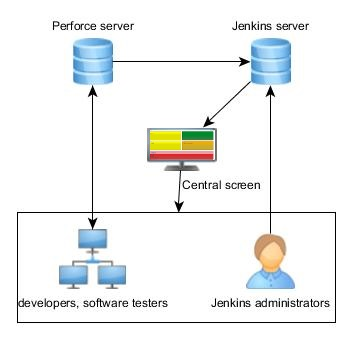
\includegraphics{images/reportingPluginEnvironmentAfter.jpg}
  \caption{L'environnement d'utilisation du plugin}
	\label{figure:reportingPluginEnvironmentAfter}
\end{figure}

Pour résumer ses caractéristiques principales, c'est un plugin qui permet :
\begin{itemize}
	\item d'afficher un écran  où chaque couleur correspond à un statut de build
	\item de rassembler les jobs par leurs préfixes communs
	\item de prendre en compte les claims
\end{itemize}

L'inconvénient est que le plugin Radiator ne permet pas de rajouter supplémentaire. Voici la liste des différents états gérés par ce plugin : 
\begin{description}
	\item[SUCCESS] Le projet compile correctement et tous les tests sont passés
	\item[ABORTED] La compilation a été arrêtée en cours d'exécution
	\item[FAILURE] Le code ne compile pas
	\item[ERROR] Erreur de l'exécution dans Jenkins
	\item[NOT BUILT] Le projet n'a pas été compilé
	\item[UNSTABLE] Des tests JUnit ne sont pas passés mais le code compile
	\item[CLAIM] Le job en échec a été claim par quelqu'un
\end{description}



Tel qu'il se présente le plugin ne permet pas de donner des informations autres que celles issues de Jenkins ou du plugin Claim. Il ne permet donc pas de donner de renseignements sur le defect associé à ce job. Tenir compte du defect permettrait de faire ressortir les régressions et autres erreurs, séparant ainsi les échecs pris en charge de ceux qui ne le sont pas.\\

\textbf{Problématique}\hfill \\ \indent
L'affichage n'est plus représentatif de la réalité, car le statut vert correspond en réalité deux status:
\begin{itemize}
	\item la réussite d'un job
	\item l'échec avec defect d'un job 
\end{itemize}

L'objet de la mission est donc de pouvoir définir un nouveau statut dans l'affichage, pouvoir choisir quand ce statut sera utilisé et pouvoir ajuster l'ordre de leurs priorités.\\
La dernière chose importante est de faire en sorte que l'utilisation du plugin soit générique et pas bornée à notre contexte d'utilisation.




\textbf{La solution propos\'{e}e}\hfill \\ \indent
Suite à la mission précédente, nous avons maintenant accès aux informations relatives aux defects (celles-ci sont enregistrées dans les archives des builds sur le serveur Jenkins), dans un fichier XML que nous avons nommé test-defects (exemple page \pageref{testdefectxml}).\\
Dans un 1\up{er} temps, et en tant qu'exercice, il faudra réaliser un plugin offrant les mêmes possibilités d'affichage des statut des builds que Radiator. C'est-à-dire rassembler les jobs par préfixe et afficher le résultat général de tous ces groupes ainsi créés sur un unique écran. Ajouté aux caractéristiques, ce plugin doit pouvoir prendre en compte les informations du plugin Claim.\\ \indent
Dans un second temps, il faudra pouvoir ajouter un ou plusieurs statut(s) supplémentaire(s) et ré-ajuster leur ordre de priorité. L'ajout de ce nouveau statut doit être générique de sorte qu'un statut quelconque puisse être ajouté.\\
Le plugin est donc capable de receuillir des informations dans des fichiers sans savoir au préalable, comment seront structurées ces données. Rappelons que, lors de l'exécution des tests, un fichier test-defect est généré contenant la liste\footnote{Au format xml} des jobs avec defect (exemple page \pageref{testdefectxml}).


\lstinputlisting[language=java,label=testdefectxml]{scripts/test-defects.xml}


\section{Organisation du travail} 
Tout au long de cette mission mon emploi du temps s'est articulé autour des meeting hebdomadaires, en fin de semaine, avec manager pour faire le point sur l'évolution du projet, présenter le produit lorsqu'il y avait une nouvelle fonctionnalité importante qui avait été implémentée et fixer les objectifs de la semaine qui allait suivre.\\
D'autre part, au minimum une heure par semaine, je faisait un \textquote{code review} avec Fabien, memebre de équipe et aussi commanditaire de ce projet.



\section{\'{E}tude préalable}
Les 1\up{er} impératifs ont été de maitriser le langage et les outils qui me permettraient de mener ce projet à terme. Je n'avais jamais entendu parler de Jenkins ou d'un quelconque logiciel d'intégration continue, et a forciori sur la manière de l'étendre. 

Avant toute étude portant sur ce que j'allais développer, je me suis renseigné sur Jenkins. Je me suis rendu sur sa documentation officiel pour en apprendre plus à ce sujet.\\

Ensuite, j'ai installé Jenkins et quelques plugins, tels qu'ils sont utilisés à SAP, de manière à me familiariser avec ceux-ci. J'ai examiner le comportement de Jenkins en l'utilisant de la manière la plus simple possible.\\

\'{E}tant un logiciel d'intégration continu, j'ai créé des projets vides (avec implémentation de tests JUnit rudimentaires) avec différents comportements lors de la compilation. Cela m'a permis d'observer le comprtement de Jenkins.\\

J'ai d'abord commencé par avoir quelques problèmes à mettre en place mon Jenkins mais ja m'en suis sorti rapidement, les problèmes n'étant que des configurations de bases sur les chemin d'accès utilisés par Jenkins. En l'occurrence le \gls{JDK} et le répertoire Maven (par souci de rapidité j'ai utilisé maven pour créer mes projets, Jenkins devais donc conna\^{i}tre son emplacement pour avoir accès à mes configurations).\\

La première chose que j'ai remarqué, et qui a été ma principale incompréhension au début, était que je ne comprenais pas la différence entre les statuts Jenkins et les statuts JUnit. Ce qui portait à confusion était leur vocubulaire, qui était en contradiction. Par exemple le statut failure de Jenkins correspond au statut Unstable de Jenkins, pour complexifier un peu la chose il existe aussi un statut failure dans Jenkins!\\
J'ai donc fait un comparatif, simplifié, de ces différents

\vspace{0.5cm}

\begin{tabular}{|l|rr|c|c|}
	\hline
  \textbf{Description du projet} 							& \textbf{Status JUnit} 	& \textbf{Statut Jenkins}\\
  \hline
  projet vide et sans test 						& NA 						& Success\\
	
	projet vide et avec test réussi			& Passed				& Success\\
  
  projet vide avec test qui échoue 		& Failure				& Unstable\\
	
  projet avec erreur de compilation 	& NA						& Error\\
  \hline
\end{tabular}

\vspace{0.5cm}

Passée cette étape d'installations et de configurations, je me suis penché sur la marche à suivre pour implémenter un plugin Jenkins.\\
La principale difficulté que j'ai eu à développer ce plugin a été de trouver l'information, il est connu sur internet que la documentation de Jenkins, lorsqu'il s'agit de l'étendre, n'est pas claire. Mais la documentation officielle\footnote{\url{https://wiki.jenkins-ci.org/display/JENKINS/Extend+Jenkins}} offre un bel éventail de ce qu'il est possible de faire, décrit les différentes technologies constituant Jenkins et offre un tutoriel trivial mais suffisant pour comprendre les bases.\\



\section{Le 1\up{er} plugin}

Je me suis d'abord rendu sur la page du tutoriel officiel de Jenkins\footnote{\url{https://wiki.jenkins-ci.org/display/JENKINS/Plugin+tutorial}} afin d'obtenir un plugin fonctionnel avec lequel je pouvais faire mes expériences (il existe un plugin \textquote{Hello world} de base, celui à partir duquel j'ai fais une grande partie de mes expérimentations). Ensuite j'ai suivi un autre tutoriel\footnote{\url{https://cleantestcode.wordpress.com/2013/11/03/how-to-write-a-jenkins-plugin-part-1/}} non-officiel mais considérablement plus riche dans lequel j'ai appris une grande partie de ce que je sais aujourd'hui sur le développement d'un plugin Jenkins.\\


\subsection{Configuration}
Pour faire mon premier plugin je me suis basé sur le archétype proposé par \gls{Maven}, le fameux \textquote{Hello world}. Maven a besoin de configurations supplémentaires dans son settings.xml\footnote{Situé dans le répertoire \texttildelow/.m2} pour pouvoir récupérer les sources relatives à Jenkins. C'est-à-dire télécharger toutes les dépendances nécessaires à la compilation.\\
Dans \textquote{pluginGroups} il faut ajouter la ligne suivante :
\begin{lstlisting}
<pluginGroup>org.jenkins-ci.tools</pluginGroup>
\end{lstlisting}
Et dans \textquote{profiles} il faut ajouter le profil suivant :
\begin{lstlisting}[language=xml]
<profile>
<id>jenkins</id>
<activation>
<activeByDefault>false</activeByDefault>
</activation>
<repositories>
<repository>
<id>repo.jenkins-ci.org</id>
<url>http://repo.jenkins-ci.org/public/</url>
</repository>
</repositories>
<pluginRepositories>
<pluginRepository>
<id>repo.jenkins-ci.org</id>
<url>http://repo.jenkins-ci.org/public/</url>
</pluginRepository>
</pluginRepositories>
</profile>
\end{lstlisting}

L'attribut de la balise \textquote{activeByDefault} est, ici, à false, parce que c'est ce qui est conseillé sur beaucoup de sites. Mais j'ai eu des problèmes, que j'ai mis un certain temps à résoudre, à cause de cet attribut.\\
Grâce à \gls{Maven} il suffit de créer un répertoire et de se placer dedans (en ligne de commande), et d'exécuter la commande ci-dessous :
\begin{lstlisting}[language=xml]
mvn hpi:create
\end{lstlisting}

\`{A} partir de là, le projet est créé et j'ai pu commencer à travailler dessus.


\subsection{Génération du squelette}
\`{A} l'exécution de cette commande, il est demandé de renseigner le groupId et l'artifactId, le groupId peut être  org.jenkins-ci.plugins et l'artifactId est le nom du plugin. Cette commande crée l'arborescence du projet ainsi que les fichiers de base. 


\`{A} la génération du squelette du plugin nous obtenons un plugin qui compile, dont l'architecture est présentée figure \ref{figure:hpiCreate} page \pageref{figure:hpiCreate}.\\

\begin{figure}[h]
  \centering
      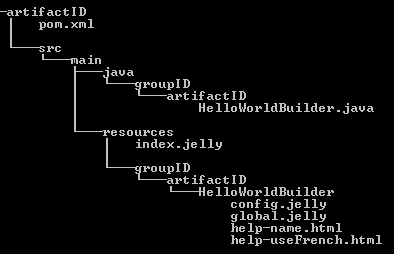
\includegraphics{images/hpiCreate.png}
  \caption{Architecture d'un plugin Jenkins généré par maven}
	\label{figure:hpiCreate}
\end{figure}


%\vspace{\stretch{1}}
Plusieurs fichiers sont générés et il est très important de conna\^{i}tre leur utilité car il est impossible de les déplacer ou de les renommer, c'est différents fichiers sont imposés par Jenkins. J'ai lis du temps à le comprendre et à chercher pourquoi mon code ne fonctionnait pas, et s'il existe un moyen de passer outre cette norme, je ne le connaîs pas encore :

\begin{tabular}{|l|p{0.7\linewidth}|}
  \hline
  \textbf{Nom du fichier} & \textbf{Description} \\
  \hline
  index.jelly & Description utilisée à la création d'une nouvelle instance du plugin \\
  config.jelly & Correspond à la page d'une instance du plugin \\
  global.jelly & Correspond à la page de configuration générale du plugin \\
  HelloWorldBuilder.java & Implémentation d'exemple du plugin \\
  help-name.html & Fichier d'aide à la configuration lorsque clic sur le symbole d'aide \\
  help-useFrench.html & Fichier d'aide à la configuration lorsque clic sur le symbole d'aide \\
  \hline
\end{tabular}


\subsection{Déploiement du squelette du plugin}
J'ai eu quelque difficulté à comprendre la logique d'intégration du plugin à Jenkins. Mais J'ai trouvé deux méthodes qui fonctionnent plutôt bien. Plutôt car j'ai rencontré certains problèmes avec ces deux procédés. \`{A} certains moments, alors je n'avais pas modifier le code, je ne pouvais plus appliquer l'une ou l'autre de ces méthodes car la compilation ne fonctionnait pas.\\
Ces deux méthodes sont les suivantes, mais je ne les aies pas appliquées très longtemps, car j'ai trouvé une bien meilleure solution pour exécuter mon plugin.\\



\textbf{Installation \textquote{\`{a} la main}}\hfill \\ \indent 
En ligne de commande et depuis la racine du projet\footnote{\`{a} l'emplacement du POM.xml}, il faut exécuter la commande suivante :
\begin{lstlisting}
mvn clean install -Pjenkins
\end{lstlisting}
Celle-ci va télécharger les sources nécessaires, les compiler, exécuter les tests et, si tout se passe bien, générer le fichier .hpi dans le dossier target.\\
Ceci fait, il faut se rendre dans Jenkins (par exemple http://localhost:8080/), s'identifier et aller dans les paramètres avancés de gestion de plugins. Ici, il faut renseigner le chemin d'accès vers le .hpi (extension reconnue par Jenkins comme étant un plugin) et terminer.\\


\textbf{Commande du plugin Jenkins de maven}\hfill \\ \indent 
En ligne de commande et depuis la racine du projet, il faut exécuter la commande suivante :
\begin{lstlisting}
mvn hpi:run -Djetty.port=8090 -Pjenkins
\end{lstlisting}
Cette commande va déployer une instances de Jenkins propre à maven, ce qui nous permet d'exécuter le plugin et le debugger. On peut très bien omettre de préciser le port utilisé si celui par défaut\footnote{port 8080} est disponible, mais il vaut mieux éviter. Une fois que le déploiement est terminé, maven signale que \textquote{Jenkins is fully up and running} nous pouvons aller voir Jenkins à l'url \emph{http://localhost:8080/jenkins} qui devrait ressembler à la figure \ref{figure:firstJenkinsWhenGenerateTheSkeletonPlugin} page \pageref{figure:firstJenkinsWhenGenerateTheSkeletonPlugin}.
\begin{figure}[!h]
  \centering
      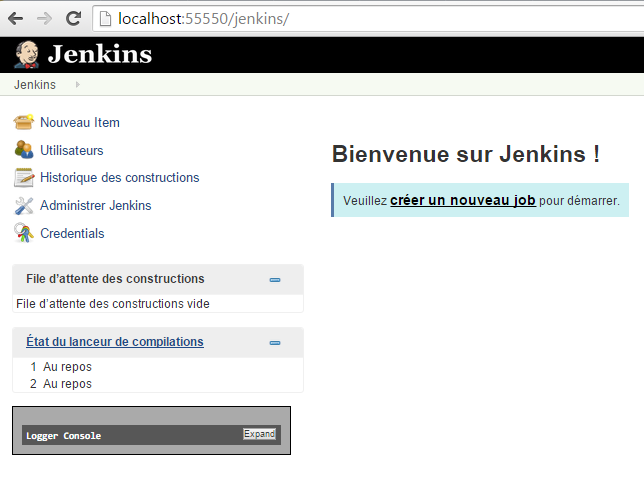
\includegraphics[width=\textwidth]{images/firstJenkinsWhenGenerateTheSkeletonPlugin.png}
  \caption{Jenkins à l'exécution de la commande maven qui l'encapsule}
	\label{figure:firstJenkinsWhenGenerateTheSkeletonPlugin}
\end{figure}




\section{Implémentation de la base du nouveau plugin}


Jenkins possède beaucoup de points d'extensions et, à cette étape, il faut déterminer lequel, ainsi que la classe à étendre. Ce choix m'a posé beaucoup de problème au début et je n'ai jamais su comment répondre à cette question. Je me suis plutôt inspiré du plugin Radiator car celui-ci fonctionnait déjà!\\

Mais plus tard, quand j'ai commencé à être plus à l'aise avec ce concept de point d'extension j'ai pu déterminer une stratégie pour savoir lequel utiliser. Mais pour cela il faut déjà conna\^{i}tre Jenkins ainsi que son code. Par exemple, dans mon cas où je souhaite afficher la liste des jobs, en parcourant la liste des points d'extensions disponibles, nous pouvons trouver \emph{View}, dont l'une de ses implémentations est \emph{ListView}; sa description étant \textquote{Displays Jobs in a flat list view}. En observant la javadoc, on peut trouver la méthode nous donnant accès aux projetx associés à la vue (figure \ref{figure:listviewJavaDoc} page \pageref{figure:listviewJavaDoc}).


\subsection{Import du code dans l'IDE}
Au début de mon travail sur l'implémentation du plugin, j'ai rencontré beaucoup de problèmes pour compiler et tester mon plugin. Il m'était d'ailleurs complètement impossible de le debugger, je perdais beaucoup de temps avec toutes les manipulations que j'étais obligé de faire juste pour tester une ligne de code.\\
Mon premier IDE pour développer ce plugin était \gls{Eclipse}. \`{A} force de perdre autant de temps et de me retrouver confronter à des problèmes n'ayant rien à voir avec l'implémentation du plugin, j'ai fini par chercher une solution avec un membre de mon équipe. Alors nous sommes allé voir un membre d'une autre équipe qui avais déjà implémenter un plugin Jenkins pour en savoir plus sur la méthode qu'il avait adoptée. Au sortir de ce meeting j'ai aussitôt installé \gls{Netbeans}, lui aussi avais rencontré les mêmes problèmes que moi et avais aussi mis un certain temps à trouver la solution.\\

L'utilisation de Netbeans (et de son plugin Jenkins) facilite l'implémentation du code et, surtout, m'a permis de me focaliser sur les problèmes liés au plugin plutôt qu'à ceux liés aux outils de développement.\\


\subsection{Implémentation de la base du plugin}

Avant de pouvoir se concentrer sur l'implementation des fonctionnalités du plugin, il faut encore savoir où écrire le code et comment nommer ses fichier. Car comme j'ne ai déjà parlé précédemment, Jenkins respecte une architecture stricte pour aller chercher les différents codes que composent ses plugin. \`{A} l'heure actuelle, je n'ai pas encore compris toutes les subtilités de cette architecture.\\
Lors de mes première expériences, je me basais sur des plugin déjà existant pour voir comment les développeurs avaient nommés leurs différents fichiers. Mais plus tard, à force de fouiller dans le code de Jenkins, j'ai découvert une méthode bien plus efficace pour répondre à cette question.\\
Pour savoir comment doit se nommer le fichier de configuration de Listview, par exemple, je suis aller chercher l'emplacement de son fichier de configuration. L'arborescence de ce fichier, dans le code de Jenkins, est illustrée figure \ref{figure:listviewJavaDoc} page \pageref{figure:listviewJavaDoc}. Il convient maintenant de copier ce fichier et de le coller dans le répertoire \emph{ressources} de notre projet. Et voilà, j'ai dans mon plugin un fichier de configuration qui sera reconnu par Jenkins et contenant le code par défaut.\\


\begin{figure}[!h]
  \centering
      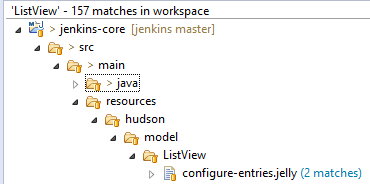
\includegraphics{images/listviewSearch.png}
  \caption{Chemin d'accès au fichier de configuration par défaut}
	\label{figure:listviewSearch}
\end{figure}



%Après quelques tests rapides, on s'aperçoit que beaucoup de code, css ou JavaScript, est exécuté lorsque l'on accède à la page. Il faut donc réinitialiser le css pour travailler dans de bonnes conditions. Premièrement, on supprime l'affichage du header, footer et side-panel de Jenkins (cf figure \ref{figure:cssInit} page \pageref{figure:cssInit}) et deuxièmement on supprime l'affichage du side-panel, après chargement de la page (cf figure \ref{figure:cssInitJS} page \pageref{figure:cssInitJS}).\\
%
%\begin{figure}[!h]
  %\centering
      %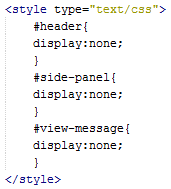
\includegraphics{images/cssInit.png}
  %\caption{Initialisation des css avant chargement}
	%\label{figure:cssInit}
%\end{figure}
%
%\begin{figure}[!h]
  %\centering
      %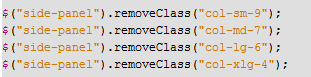
\includegraphics{images/cssInitJS.png}
  %\caption{Initialisation des css après chargement}
	%\label{figure:cssInitJS}
%\end{figure}


\section{Travail réalisé}

\`{A} partir du moment où j'ai compris la logique d'implémentation d'un plugin Jenkins, j'ai enfin pu me concentrer sur ma mission.\\
Je me suis fixé comme premier objectif d'afficher une nouvelle vue que j'aurais implémentée moi-même : typiquement un écran blanc n'affichant que chaine de caractère issue de mon implémentation \gls{Java}, cet objectif simple permet de faire le lien entre l'interface graphique, codée en jelly, et le code \gls{Java}.\\
J'ai trouvé dans la documentation de Jenkins les quelques éléments qui allais me permettre de réaliser ceci : les deux objets \textquote{it} et \textquote{from}, ces deux objets me permettent d'accéder à la classe principale de mon plugin. Il permettent d'accéder aux méthodes et propriétés de l'instance du plugin.\\
Les appels ne se font pas de la même manière mais se basent toujours sur ces deux objets.\\

L'accès aux attributs se fait en l'appelant simplement de la manière suivante :
\begin{lstlisting}
<j:set var="maVariable" value="${from.maPropiete}">
<j:set var="maVariable2" value="${from.maPropiete2}">
\end{lstlisting}
Cela permet de d'initialiser une variable jelly et de lui donner la valeur de la proprité souhaitée.
L'accès aux méthode se fait un peu différemment :
\begin{lstlisting}
%<j:invoke var="maVariable" on="${from}" method="nomDUneMehode">
\end{lstlisting}
Et de la même manière, cette exemple permet d'appeler une méthode depuis l'objet from dont le retour est placé dans la variable jelly.\\

La logique d'implémentation du jelly est assez simple en soit et je me la suit rapidement appropriée. J'ai trouvé très agréable d'utiliser aussi facilement mon \gls{Java} depuis mon jelly, car celui-ci est implémenté côte-à-côte avec le code html.\\

Grâce à ce code très simple, j'ai pu afficher ce que je voulais dans mon jelly en utilisant la notation jelly : \$\{maVariableJelly\}\\




\subsection{Construction d'une architecture en corrélation avec l'affichage souhaité}
Pour accéder aux différents jobs de Jenkins, il suffit de faire appel à l'une des méthodes de la classe mère : getItems(), retournant une liste de TopLevelItem. Toutes ces informations sont disponibles dans la javadoc du produit que j'ai longuement parcourue pour comprendre son fonctionnement. Mais malheureusement cet objet ne correspond pas vraiment à l'utilisation que je voulais en faire. J'ai donc créé une nouvelle classe : ProjectWrapper, comprenant cet objet ainsi que d'autres, plus spécifiques à mon plugin.\\


La méthode \gls{Java} que j'ai donc implémenté est la suivante :\\
\begin{lstlisting}
public List<ProjectWrapper> getSelectedJobs() {
        List<ProjectWrapper> jobs = new ArrayList<ProjectWrapper>();
        ProjectWrapper project;
        for ( TopLevelItem item : super.getItems() ) {
            if (item instanceof AbstractProject) {
              project = new ProjectWrapper(this, (AbstractProject) item);
              if (!project.getAbstractProject().isDisabled()) {
                 jobs.add(project);
            }
        }
    }
    return jobs;
}
\end{lstlisting}
		
Grâce à cette liste ainsi obtenue je pouvais avoir accès à la liste de mes jobs depuis mon interface graphique.\\
La plus grande difficulté que j'ai rencontré pour pouvoir afficher les jobs était de les afficher tels que je le voulais, autrement regroupés par préfixes qu'ils avaient en commun.\\

J'ai donc passé beaucoup de temps à construire une architecture qui me permttrait de réaliser cela, et je suis donc arrivé à créer un certain nombre de classes me permettant ceci.\\
Je développe en \gls{Java}, et pour respecter au mieux la logique de la programmation orientée objet, j'ai fais en sorte que mes objets \gls{Java} représentent vraiment les différents éléments de mon inerface graphique.\\
L'objet central de la logique que j'ai implémenté est le dashboard, celui-ci contenant la liste des différentes vues qui le compose, je l'ai nommé Dashboard!\\ Ensuite, chacune des vues intégrée à mon dashboard sont caractérisées par un préfixe (point commun à tous les projets qu'elle contient), un état dominant (état qui fera que la vue s'affiche de telle ou telle couleur) et d'une liste de projets. J'ai nommé cet objet ViewEntry.\\
Et pou finir, chacun des projets contenus dans une vue est caractérisé par un préfixe et un résultat personnalisé (personnalisé car un projet ne peut avoir qu'un seul état mais j'ai trois sources différentes pouvant influencer cet état : Jenkins, le plugin Claim ou un état choisi par l'utilisateur). Je l'ai nommé ProjectWrapper.\\
Chacun de ces objets possède un ensemble de comportement qui leur est propre. Par exemple, dans le cas du Dashboard, trier une liste de projets en une liste de vues (où tous les projets d'un vue on le même préfixe). Dans le cas de la ViewEntry, pouvoir ajouter un projet a sa liste de projets. Et dans le cas du ProjectWrapper, pouvoir fournir son préfixe s'il en a un, ou son statut.\\

Le diagramme de classe représentant cette architecture que j'ai ainsi construite est illustré page \pageref{figure:myDash}, et j'ai représenté l'algorithme me permettant d'obtenir mon Dashboard à partir d'une liste de ProjectWrapper page \pageref{figure:dashboardGenesis}



\begin{figure}[H]
  \centering
      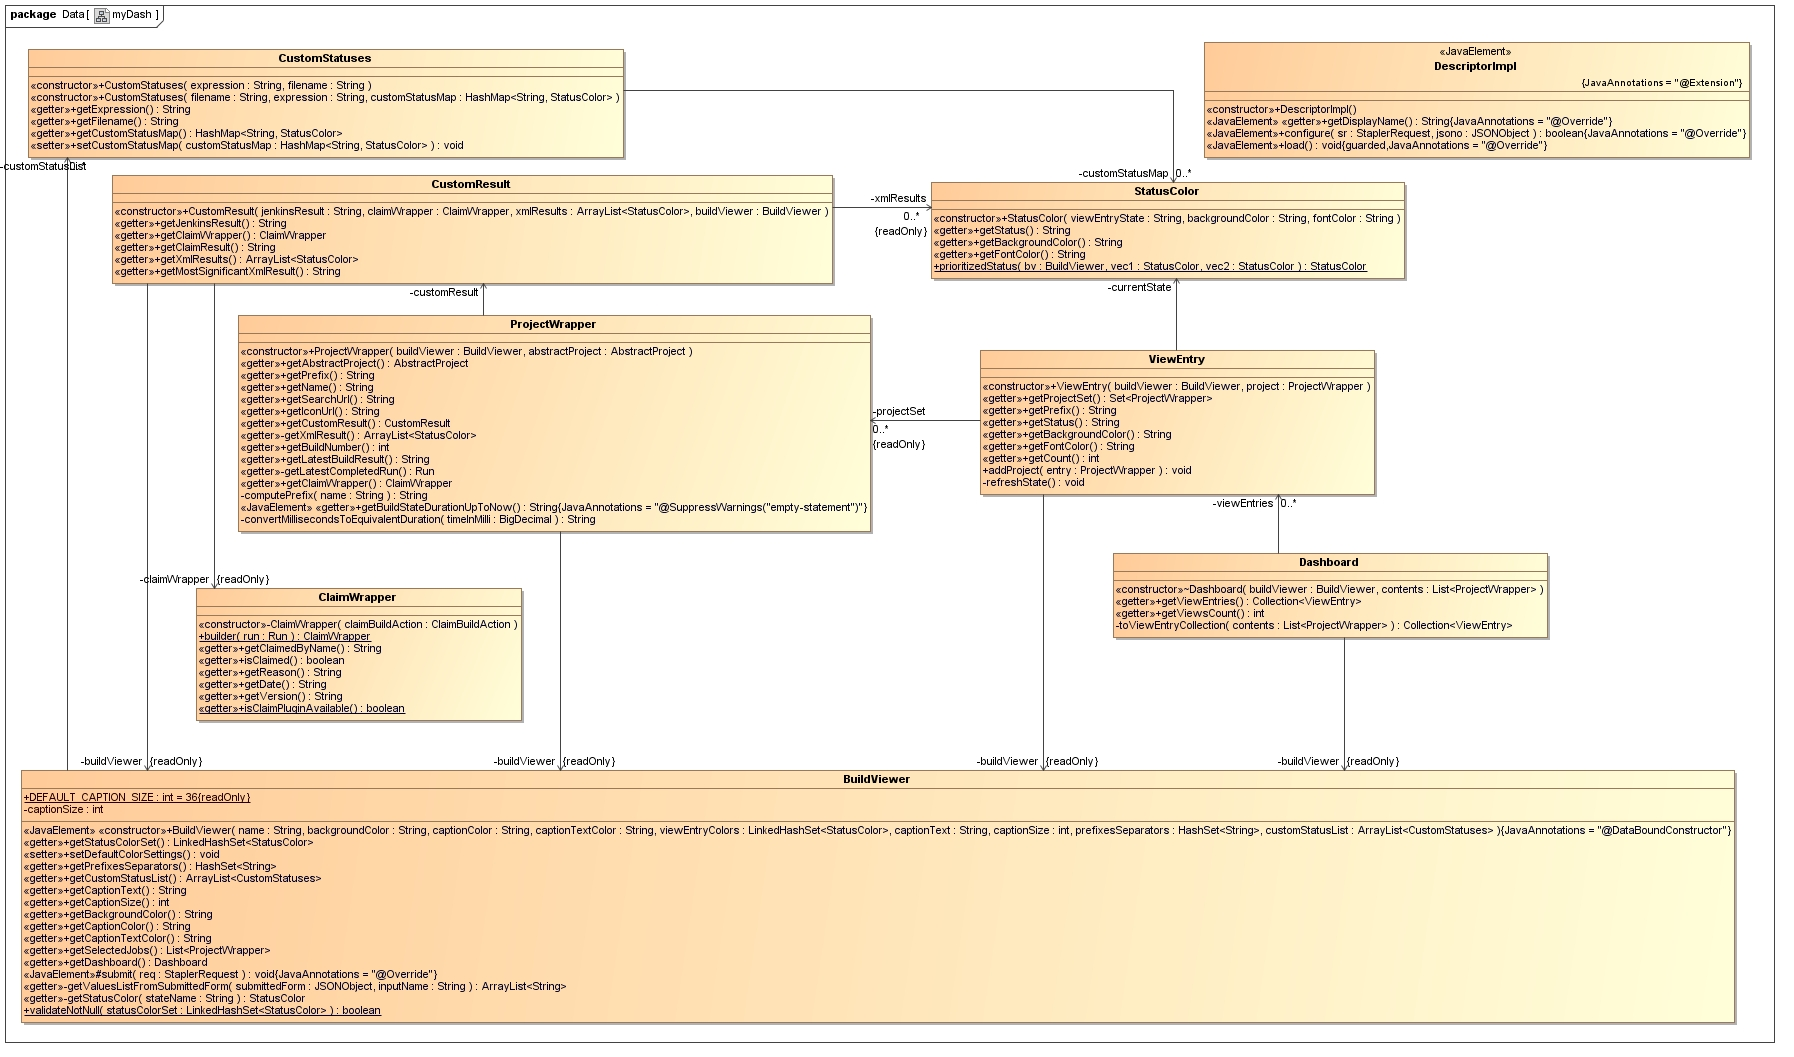
\includegraphics[width=\textheight,angle=90]{images/myDash.jpg}
  \caption{Diagramme de classe du plugin réalisé}
	\label{figure:myDash}
\end{figure}



\begin{figure}[H]
  \centering
      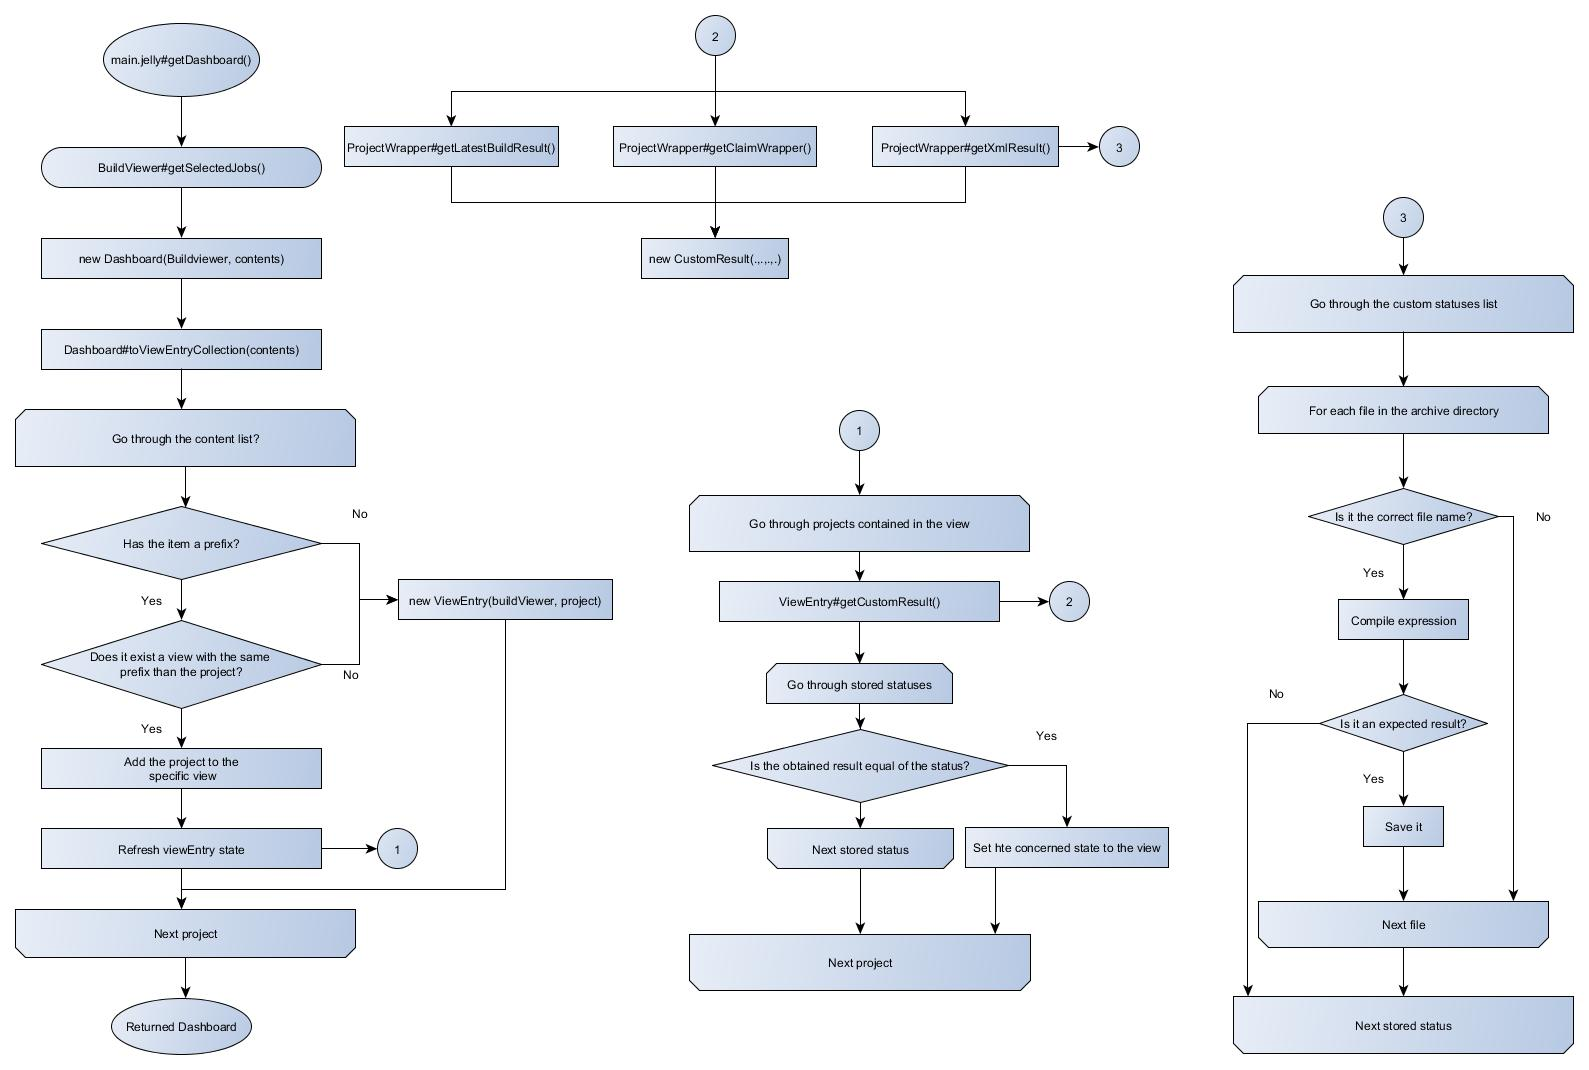
\includegraphics[width=\textheight,angle=90]{images/dashboardGenesis.jpg}
  \caption{Algorithme de création du Dashboard}
	\label{figure:dashboardGenesis}
\end{figure}


\subsection{Affichage des jobs dans l'interface graphique}

Les objets \gls{Java} représentatifs de mes vues étant implémentés, l'objectif était maintenant de pouvoir les afficher correctement. Il me fallait donc dimensionner mes vues en fonction, d'une part du nombre de vues, et d'autre part, de la taille de l'écran.\\
J'ai d'abord voulu essayer de dimensionner les vues directement à l'affichage, dans l'interface graphique. Cela fonctionnait très bien, puisqu'à partir du Dashboard je pouvais récupérer les nombre de vues générées et ainsi les dimensionner en fonctions de la taille de l'écran. L'inconvénient de cette méthode était que la taille de l'écran n'étant pas accessible depuis le jelly j'étais obligé d'attribuer moi-même la valeur de la taille de l'écran. Cela ne m'a pas posé de problème au début mais lorsque j'ai essayé le plugin sur d'autre écrans, plus petits ou plus grands, le dimensionnement ne pouvait plus fonctionné.\\
J'ai donc opté pour la solution javascript. Je ne connaissais que très peu ce langage avant cet épisode et j'ai dû passer un peu de temps à l'apprendre. Ce qui a été plutôt rapide car je ne me contentais que de mettre en forme mes éléments html en modifiant mes feuilles de styles.\\

La solution la plus simple pour déterminer la largeur et la hauteur d'une vue a été, d'abord, de considérer que celles-ci seraient toutes de la même taille, et ensuite de baser ce calcul sur les dimensions du dashboard (celui-ci étant configuré de manière à occuper 100\% de l'espace disponible).\\
Concrètement, mon algorithme de dimensionnement est le suivant :
\begin{itemize}
	\item Je calcule le carré minimum pouvant acceuillir toutes mes vues (4 vues impliquent un carré de 2, 6 vues impliquent un carré de 3, ...)
	\item J'en déduis mon nombre de lignes en divisant le total des vues par le carré trouvé ( 6 \textbackslash 3 = 2 implique 2 lignes)
	\item Si le résultat de la division n'est pas entier je rajoute une ligne (pour 7 vues j'aurais 2 lignes de 3 vues et 1 autre de 1)
	\item De ces valeurs j'en déduis les dimensions de mes vues
\end{itemize}

J'ai appliqué quelques coefficients tenant compte du fait que les marges entre les vues sont constantes.\\
Le code javascript ainsi développé est ci-dessous :

\begin{lstlisting}
%breadcrumbarheight = $('div#breadcrumbBar').css("height").split("px")[0];
%h=h-breadcrumbarheight-15;
%var countOfViews = document.getElementById("hiddenCountOfViews").value;
%var captionSize = document.getElementById("hiddenCaptionSize");
         %
%if(captionSize==null){
	%captionSize=0;
%}else{
  %captionSize=captionSize.value;
%}
%xdash = 0;
%while (countOfViews &gt; xdash * xdash) {
  %xdash++;
%}
%var countOfRows = Math.floor(countOfViews / xdash);
        %
%if((countOfViews % xdash)!=0){
  %countOfRows = countOfRows +1;
%}
%var viewheight = ((h - captionSize) / countOfRows) - 4*countOfRows;
%var viewwidth = (w / xdash) - 5*xdash;
\end{lstlisting}

Ce code fonctionnait très bien et j'ai donc voulu essayer mon plugin dans un contexte d'utilisation réelle, c'est-à-dire en intégrant mon plugin à Jenkins en utilisant le fichier d'installation .hpi.\\
J'ai eu la surprise de constater que, malgré que le dimensionnement se passait bien, tout le contenu de mon dashboard était décalé vers la droite d'une certaine distance qui restait la même quelle que soit la dimension de l'écran que j'utilisais.\\
J'ai passé beaucoup de temps à chercher ce qu'il se passait, sans comprendre d'où cela pouvait venir. J'ai cherché dans le plugin Radiator s'il prenait en compte autre chose que j'avais ignoré, mais sans résultat. \\
Je n'ai pas investigué longtemps dans le code car je ne pouvais rien trouver de cette manière. J'ai donc lancé les deux versions de Jenkins que j'avais, l'une en exécutant le plugin depuis Jenkins (où tout se comportait comme prévu) et l'autre (où le problème avait lieu).\\
De ces deux versions différentes j'ai analysé les deux codes sources des pages et ai écrit un petit programme java me permettant de faire ressortir les différences. Après un certain temps d'analyse j'ai remarqué qu'il y avait une différence entre les deux versions. L'un des éléments html, commun aux deux versions, ne possédait pas les mêmes classes. Je suis donc allé dans le code de Jenkins pour voir a quoi correspondait ce code, il s'agissait en fait d'une portion de l'écran (précisément le \textquote{side-panel}) qui était réservé au menu de Jenkins, et si le plugin Radiator ne rencontrait pas ce problème c'est que celui-ci avait été développé sur une version antérieure dans laquelle le positionnement ne se faisait pas de la même manière\footnote{voir \url{https://issues.jenkins-ci.org/browse/JENKINS-29659}}.\\
\'{E}tant au courant de la raison exacte du problème que j'ai rencontré j'ai pu le corriger en quelques lignes de JQuery ci-dessous :\\
\begin{lstlisting}
$("side-panel").removeClass("col-sm-9");
$("side-panel").removeClass("col-md-7");
$("side-panel").removeClass("col-lg-6");
$("side-panel").removeClass("col-xlg-4");
\end{lstlisting}

J'ai de nouveau testé mon plugin tel qu'il le serait réellement, tout fonctionnait comme je le désirais.\\
Ce problème a perduré longtemps parce que, ne sachant pas comment le résoudre, je l'ai laissé de côté en attendant d'avoir une meilleure idée. Avec le temps, accumulant de l'expérience tant avec les outils que j'utilisais qu'avec les langages que j'utilisais, j'ai eu cette idée qui m'a permis de résoudre ce problème en moins de deux heures.\\

%claim? priorité des status?

\subsection{Personnalisation des statuts}

J'avais donc à cette étape là un plugin me permettant d'afficher tous les jobs regroupés par préfixes dans des vues de la couleur représentative du statut jugé prioritaire par l'utilisateur. \`{A} ce niveau d'avancement de mon projet, le plugin possède déjà toutes les fonctionnalités de l'ancien plugin Radiator. \`{A} la seule différence que mon plugin permet de configurer l'ordre des priorités.\\
J'en arrivais maintenant à la fonctionnalité principale de mon plugin, raison d'être de mon projet : pouvoir configurer ses propres statuts se basant sur des fichiers xml.\\
La première question était de savoir comment récupérer ces fichiers xml.\\
La deuxième question, comment en extraire les résultats.\\
La troisième question, comment faire correspondre un résultat à un statut.\\

Lors de l'exécution des tests tous les fichiers générés sont enregistrés dans un répertoire d'archive (y compris les fichiers des résultats JUnit) je devais donc savoir comment y accéder. Pour répondre à cette question j'ai simplement récupérer toutes les informations disponibles dans un projet Jenkins jusqu'à tomber sur le répertoire du projet, duquel je suis parti pour me trouver dans le répertoire \textquote{archive}, le code me permettant d'avoir un objet File représentatif de ce dossier est le suivant :\\
\begin{lstlisting}
File files = new File(abstractProject.getBuildDir().getAbsolutePath() + "\\" + run.getId() + "\\archive");
\end{lstlisting}

Je peux maintenant tester l'existence d'un fichier (dont le nom est renseigné par l'utilisateur). Je devais pouvoir extraire une information de fichier, la méthode la plus simple, en considérant que j'ai affaire à un fichier xml, est d'utiliser un XPath pour obtenir mon information.\\
Je n'avais jamais utilisé cette technologie, bien que j'en connaissais son existence. Après quelques expérimentations j'ai obtenu un code fonctionnant bien me permettant, pour l'instant, de récupérer la valeur d'un attribut, que je pouvais retourner.\\

La vraie difficulté de cette partie à été d'implémenter une table dont les éléments sont \textquote{drag'n'droppable}. J'ai essayé un certain nombre de technologies, certaines correspondant tout à fait et étaient très faciles à utiliser mais dont le simple import de la libraire rendait le plugin inutilisable.\\
J'ai donc choisi de ne pas utiliser de librairie pour implémenter mon \textquote{drag'n'drop} et ai tout fait moi-même. Le \textquote{drag'n'drop}, uniquement des lignes d'un tableau étant plutôt facile à implémenter, j'ai pris le temps de le faire pour en retirer un résultat très satisfaisant.\\
Une fois la table implémentée il fallait, d'une part, pouvoir ajouter et supprimer des lignes, et d'autre part, que la modification de la table des statuts ait une influence sur la table des statuts personnalisés. Ceci à été assez difficile car l'ajout d'une ligne dans la table est exécuté par un code javascript contenant le code à ajouter. Ce qui nécessitait de modifier le code à deux endroits différents à la moindre modification de la table. Ensuite, les éléments à ajouter dans la ligne à ajouter, comme son identifiant, sont difficilement récupérables du simple fait que la génération ne se passe pas au même moment. Quand une table est générée, le jelly s'occupe d'incrémenter un variable pour identifier les lignes, mais quand je veux ajouter une ligne, non seulement, cette variable n'existe plus, mais aussi, je me trouve alors dans un code javascript.\\
J'ai donc passé beaucoup de temps à mettre en relation tous ces éléments, de manière à ce que l'interface graphique que l'utilisateur a sous les yeux soit complètement dynamique.










\section{Les échos de mon projet}


Lorsque je suis arrivé à un résultat satisfaisant il devenait nécessaire de présenter mon travail aux autres membres de mon équipe. J'ai donc préparer un PowerPoint pour étayer mes propos.\\
Ma première présentation, devant l'équipe ST Automation, s'est déroulée le jeudi 13 août 2015.\\
Mon auditoire n'a pas vraiment compris les détails de ce que je disais car je suis allé trop vite au début de la présentation et je n'ai pas pris le temps de clairement définir le domaine d'utilisation de mon plugin. De plus, une majorité des personnes présentes n'utilisait pas le vocabulaire que j'utilisais. L'autre point important, favorisant une certaine incompréhension de mon auditoire, était que je n'avais pas détaillé le contexte actuel, c'est-à-dire d'une part, l'utilisation du plugin Radiator, et d'autre part, la mécanique que j'ai mise en place précédemment pour obtenir un statut JCWB me permettant de le réutiliser. Pour terminer cette présentation, je n'ai pas fait de simulation de mon produit pour montrer à quoi il ressemble, cela aurait permis à mon auditoire de visualiser mon travail.\\
J'ai fait un seconde présentation, devant l'équipe SDK cette fois-ci. J'avais pris le temps de faire de nouveau slides me permettant de m'attarder un peu plus sur le contexte antérieur à mon projet et à la problématique, rencontrée. J'ai aussi fait la démonstration du plugin précédent et de mon plugin pour marquer les différences. Mon auditoire à beaucoup mieux compris le contexte de mon plugin. Le point que je devais encore améliorer était de bien séparer les différentes parties : avant, quel problème; aujourd'hui, quelle solution; dans le futur, toutes les fonctionnalités désirées.\\
Une autre présentation est prévue mais celle-ci n'est pas encore planifier à l'heure où j'écris ce rapport.\\
Je ferai beaucoup plus attention à présenter le contexte et je présenterai la problématique avec beaucoup plus soin de manière à ce que mon auditoire puisse comprendre tout le contexte dans lequel s'inscrit l'utilisation de mon plugin, et ainsi, son intérêt.\\



